\section{法兰盘三视图}

{\bfseries 知识目标}
\begin{itemize}
\item 掌握回转体三视图规律
\end{itemize}

{\bfseries 技能目标}
\begin{itemize}
\item 能够应用三视图对应关系,运用AutoCAD绘制回转体的三视图
\end{itemize}

图\ref{fig:falanpanlititu}所示为工业中应用泛用于管道连接的法兰盘零件的简化形式。本任务主要是让读者了解并掌握回转体三视图表述方式,实现应用AutoCAD进行回转体类零件的三视图绘制的技能目标。
\begin{figure}[htbp]
\centering
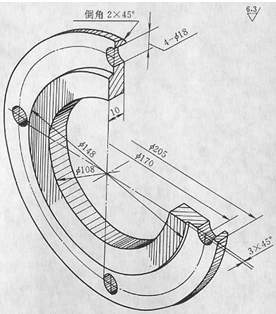
\includegraphics[scale=1]{fananlititu.png}
\caption{法兰盘}\label{fig:falanpanlititu}
\end{figure}
\subsection{绘制法兰盘主视图}
法兰盘整体是由两个圆筒叠加构成的,并具有四个用于安装的联接孔。我们先选择最能够表达的其形状的特征的方向作为其主视图。

具体绘图过程如下:

第一步:先定义图层,如图\ref{fig:falantucen}所示。
\begin{figure}[htbp]
\centering
\begin{floatrow}
\ffigbox{\caption{法兰盘图层定义}\label{fig:falantucen}}
{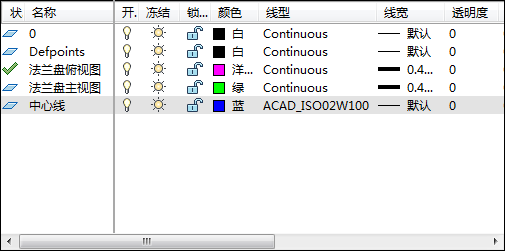
\includegraphics[scale=0.5]{falantucen.png}}
\ffigbox{\caption{法兰盘主视图}\label{fig:falanzhushitu}}{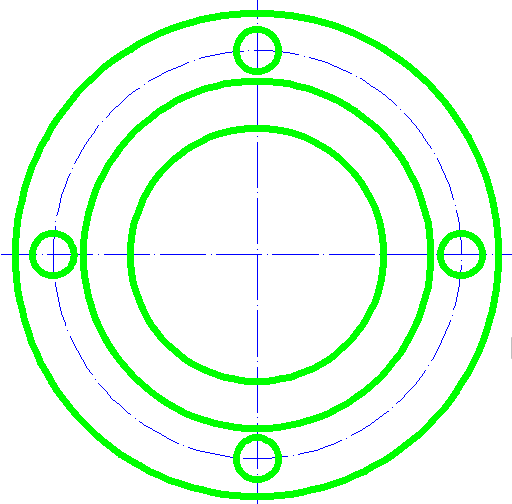
\includegraphics[scale=0.25]{falanzhushitu.png}}
\end{floatrow}
\end{figure}

第二步:绘制中心线,并完成主视图,如图\ref{fig:falanzhushitu}所示。
\begin{figure}[htbp]
\centering
\begin{floatrow}
\ffigbox{\caption{法兰盘俯视图}\label{fig:falanfushitu}}{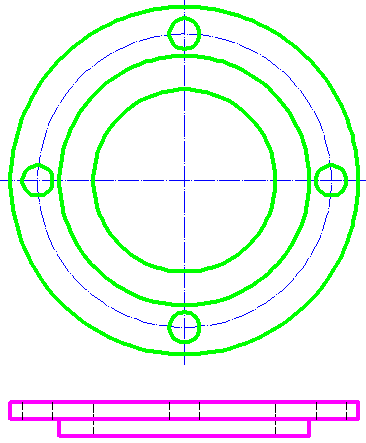
\includegraphics[scale=0.3]{falanfushitu.png}}
\ffigbox{\caption{法兰盘三视图}\label{fig:falansanshitu}}{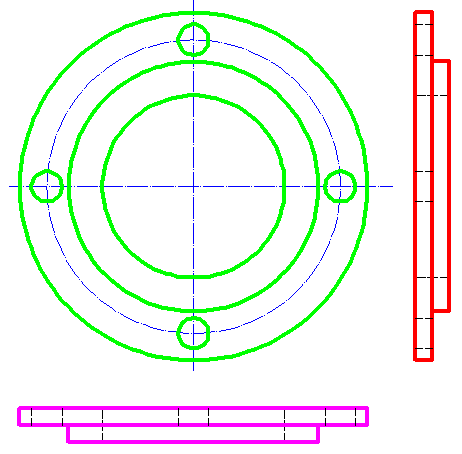
\includegraphics[scale=0.3]{falansanshitu.png}}
\end{floatrow}
\end{figure}

\subsection{绘制法兰盘俯视图}
第一步:先利用长对正关系,确定定俯视图中对应部件的投影关系。

第二步:根据\ref{fig:falanpanlititu}所示尺寸绘出俯视图,如图\ref{fig:falanfushitu}所示。

\subsection{绘制法兰盘左视图}
利用主、左高平齐,俯左宽相等的对应关系绘制左视图的相关部分,最终形成三视图如图\ref{fig:falansanshitu}所示。

\endinput